\documentclass{beamer}
\usetheme{Madrid}
\usecolortheme{default}

\usepackage[utf8]{inputenc}
\usepackage[T1]{fontenc}
\usepackage{listings}
\usepackage{xcolor}
\usepackage{booktabs}
\usepackage{amssymb}

\definecolor{codegray}{gray}{0.5}
\definecolor{codeblue}{rgb}{0.0,0.0,0.6}
\lstdefinestyle{verilog}{
  language=Verilog,
  basicstyle=\ttfamily\scriptsize,
  keywordstyle=\color{codeblue}\bfseries,
  commentstyle=\color{codegray}\itshape,
  numbers=none,
  breaklines=true,
  showstringspaces=false,
}
\lstset{style=verilog}

\title[RISC-V Pipeline + RVC]{Procesador RISC-V Pipelined con Extensión C}
\subtitle{Pipeline, Hazard Unit e Instrucciones Comprimidas}
\author[Ildefonso, Paucar, Rosillo]{%
  \begin{tabular}[t]{c}Ildefonso Santos\\Steve Andy\end{tabular}
  \and
  \begin{tabular}[t]{c}Paucar Barrios\\Miguel Luis\end{tabular}
  \and
  \begin{tabular}[t]{c}Rosillo Rodríguez\\Marcelo Mateo\end{tabular}
}
\institute{UTEC --- Arquitectura de Computadoras}
\date[]{Julio 2026}

\makeatletter
\setbeamertemplate{footline}{%
  \leavevmode%
  \hbox{%
  \begin{beamercolorbox}[wd=.5\paperwidth,ht=2.25ex,dp=1ex,center]{author in head/foot}%
    \usebeamerfont{author in head/foot}\insertshortauthor
  \end{beamercolorbox}%
  \begin{beamercolorbox}[wd=.5\paperwidth,ht=2.25ex,dp=1ex,leftskip=5em,rightskip=1ex]{title in head/foot}%
    \usebeamerfont{title in head/foot}\insertshorttitle\hfill
    \insertframenumber{} / \inserttotalframenumber
  \end{beamercolorbox}}%
  \vskip0pt%
}
\makeatother

\AtBeginSection[]
{
  \begin{frame}
    \frametitle{Contenido}
    \tableofcontents[currentsection]
  \end{frame}
}

\begin{document}

\frame{\titlepage}

\begin{frame}{Contenido}
  \tableofcontents
\end{frame}

% ============================================================
\section{Proceso de construcción}
% ============================================================

\begin{frame}{Metodología: incremental, por entregas}
  \begin{itemize}
    \item<1-> \textbf{E1 (5 pts)}: pipeline base de 5 etapas + Hazard Unit
      (forward/stall/flush) + ISA RV32I (24 instrucciones).
    \item<2-> \textbf{E2 (4 pts)}: extensión C, parte 1 --- 11 instrucciones
      comprimidas de ALU/registro-inmediato.
    \item<3-> \textbf{E3 (3 pts)}: extensión C, parte 2 --- 10 instrucciones
      de memoria y control de flujo.
  \end{itemize}
  \vspace{0.3cm}
  \begin{block}{Ciclo por fase}
    implementar $\to$ programa de prueba $\to$ testbench $\to$ waveform
    $\to$ siguiente fase. Este patrón se ve en detalle en los próximos dos
    capítulos.
  \end{block}
\end{frame}

% ============================================================
\section{Pipeline y Hazard Unit}
% ============================================================

\begin{frame}{El pipeline base: 5 etapas}
  \begin{columns}
    \column{0.55\textwidth}
    \begin{itemize}
      \item<1-> \textbf{Fetch}: PC, memoria de instrucciones
      \item<2-> \textbf{Decode}: banco de registros, extend
      \item<3-> \textbf{Execute}: ALU, cálculo de saltos
      \item<4-> \textbf{Memory}: memoria de datos
      \item<5-> \textbf{Writeback}: escritura al banco de registros
    \end{itemize}
    \column{0.45\textwidth}
    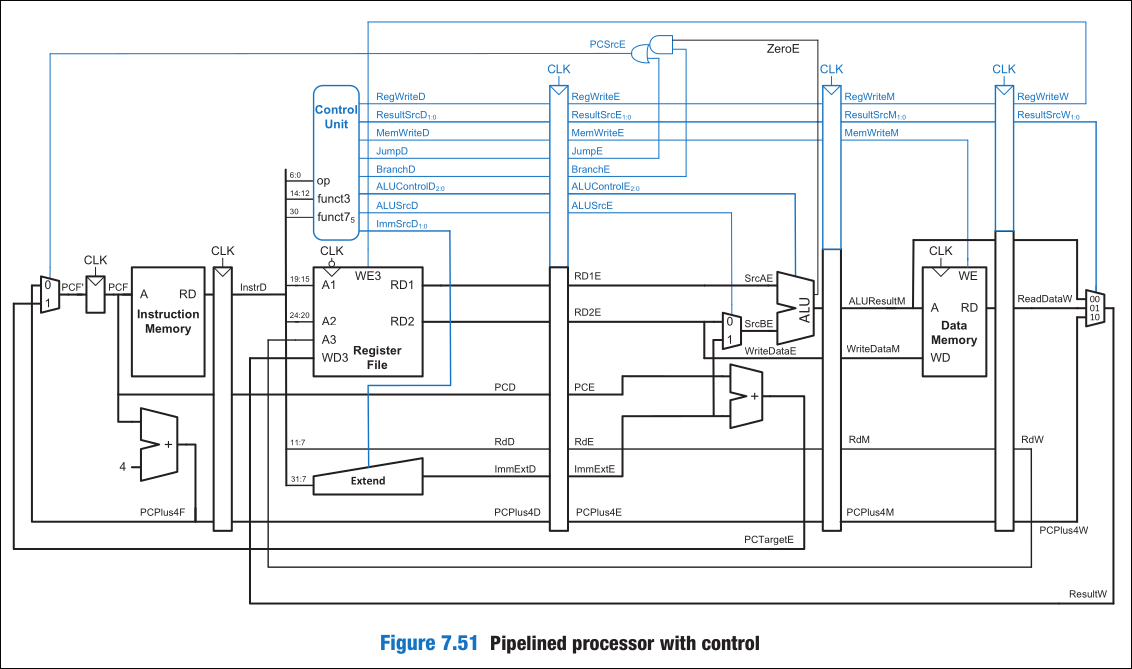
\includegraphics[width=\textwidth]{../pipeline_diagram.png}
  \end{columns}
\end{frame}

\begin{frame}{Riesgos (\textit{hazards})}
  \begin{block}{El precio de segmentar}
    Varias instrucciones en vuelo a la vez $\Rightarrow$ los datos y saltos no
    siempre están listos a tiempo.
  \end{block}
  \begin{itemize}
    \item \alert{De datos (RAW)}: una instrucción usa un resultado que otra
      anterior aún no escribió. Caso crítico: \textit{load-use}.
    \item \alert{De control}: los saltos se resuelven en Execute, pero ya se
      captaron instrucciones secuenciales de más.
    \item \alert{Estructurales}: evitados por diseño (imem/dmem separadas,
      regfile lee y escribe en el mismo ciclo).
  \end{itemize}
\end{frame}

\begin{frame}{Forward: adelantar el dato}
  El programa quiere usar un resultado apenas calculado en la instrucción
  siguiente; sin \textit{forwarding} lee el valor viejo del banco de
  registros.
  \begin{columns}
    \column{0.5\textwidth}
    \centering \scriptsize Sin Hazard Unit (falla)\\
    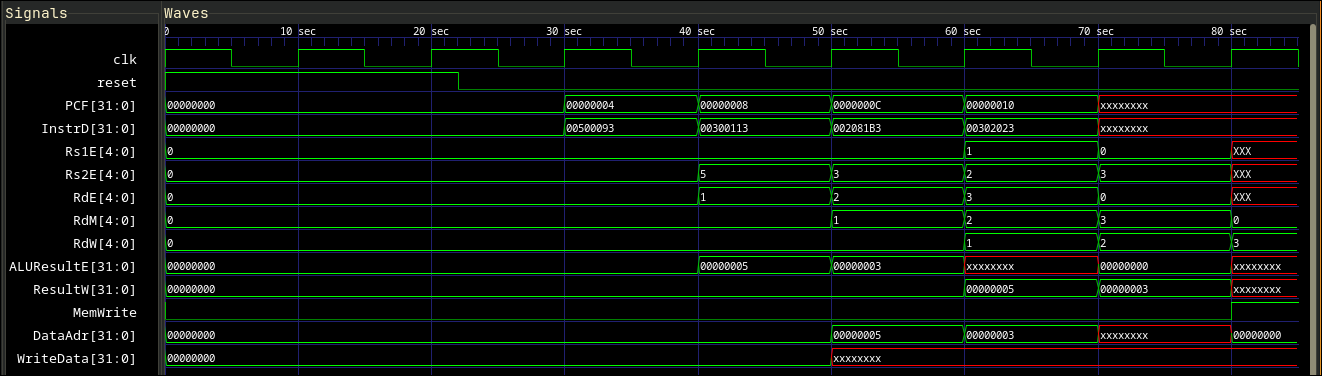
\includegraphics[width=\textwidth]{../hazard_forward_nohu.png}
    \column{0.5\textwidth}
    \centering \scriptsize Con Hazard Unit (\texttt{ForwardAE/BE})\\
    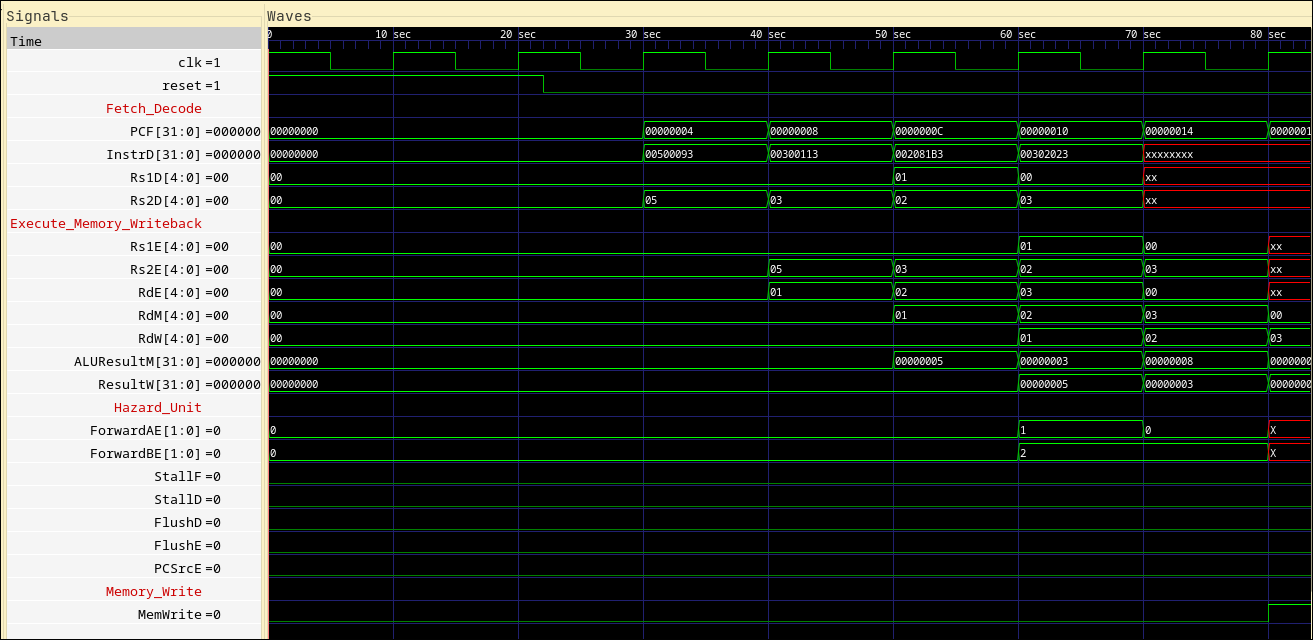
\includegraphics[width=\textwidth]{../hazard_forward_waveform.png}
  \end{columns}
\end{frame}

\begin{frame}{Stall: el caso \textit{load-use}}
  El programa quiere usar un valor que recién se está leyendo de memoria; no
  se puede resolver solo con \textit{forwarding} --- hay que detener el
  pipeline un ciclo.
  \begin{columns}
    \column{0.5\textwidth}
    \centering \scriptsize Sin Hazard Unit (falla)\\
    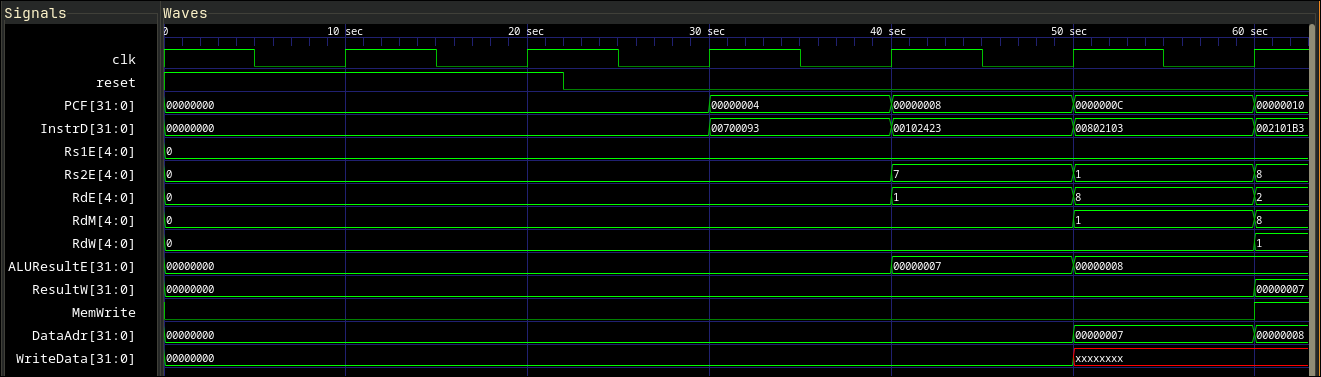
\includegraphics[width=\textwidth]{../hazard_stall_nohu.png}
    \column{0.5\textwidth}
    \centering \scriptsize Con Hazard Unit (\texttt{StallF/D})\\
    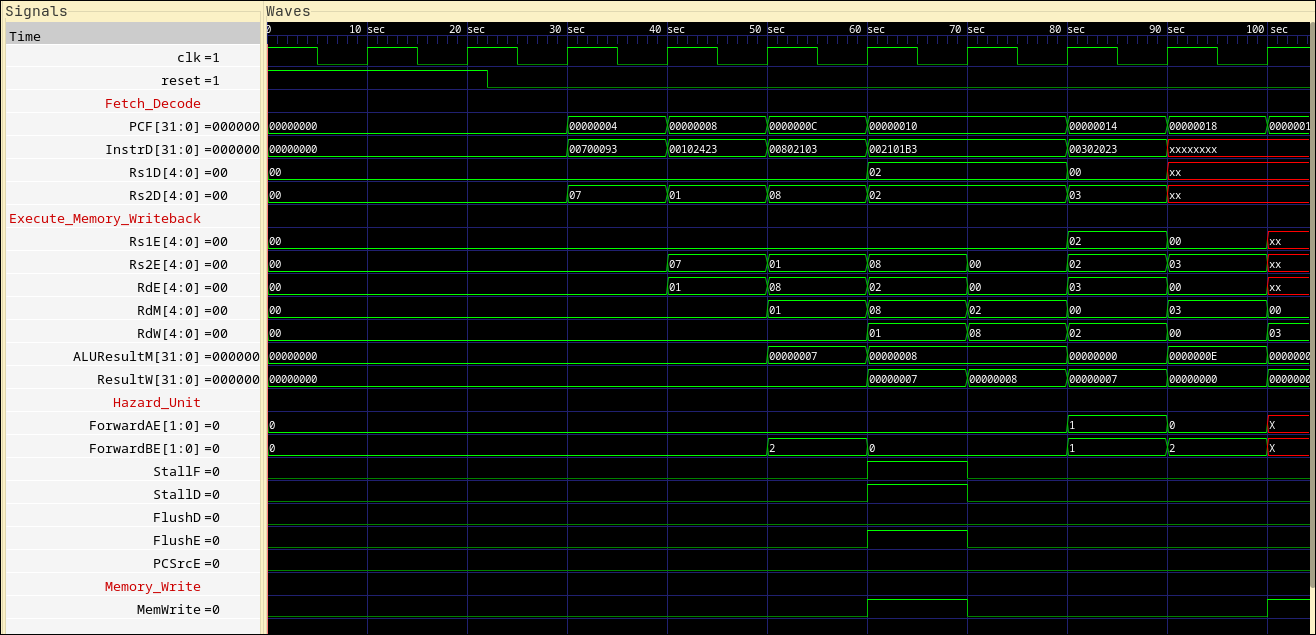
\includegraphics[width=\textwidth]{../hazard_stall_waveform.png}
  \end{columns}
\end{frame}

\begin{frame}{Flush: descartar tras un salto}
  El programa tiene un salto/branch; las instrucciones ya cargadas en el
  pipeline detrás del salto son incorrectas y hay que descartarlas.
  \begin{columns}
    \column{0.5\textwidth}
    \centering \scriptsize Sin Hazard Unit (falla)\\
    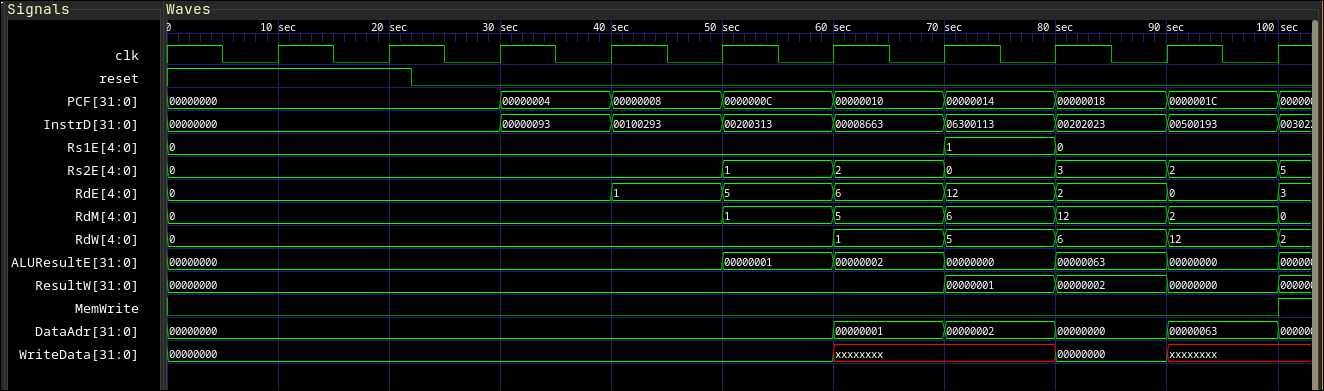
\includegraphics[width=\textwidth]{../hazard_flush_nohu.png}
    \column{0.5\textwidth}
    \centering \scriptsize Con Hazard Unit (\texttt{FlushD/E})\\
    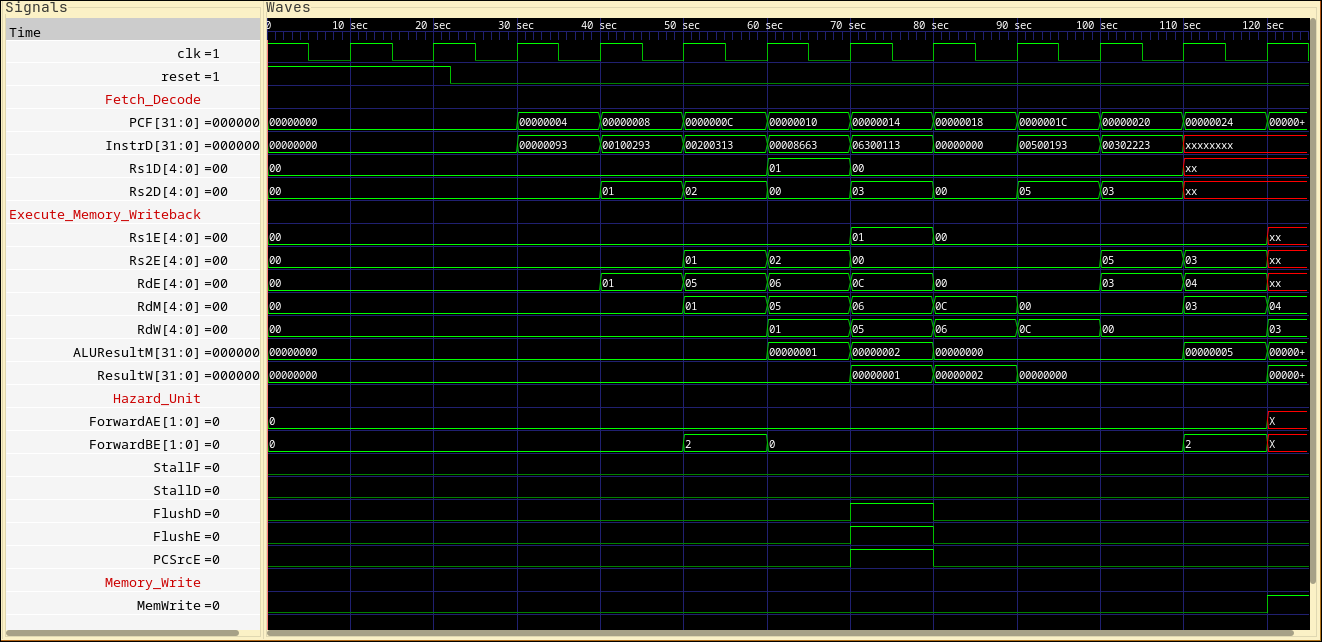
\includegraphics[width=\textwidth]{../hazard_flush_waveform.png}
  \end{columns}
\end{frame}

\begin{frame}{Datapath final: implementación de instrucciones}
  \centering
  \includegraphics[width=0.98\textwidth]{../datapath_final.pdf}
  \vspace{2mm}

  {\scriptsize En \textcolor{red}{rojo}: adiciones propias sobre el pipeline
  base --- \texttt{Jalr}, \texttt{funct3E}, \texttt{ALUControl} de 4 bits,
  mux de destino \texttt{jalr}.}
\end{frame}

% ============================================================
\section{Extensión C: instrucciones comprimidas}
% ============================================================

\begin{frame}{¿Qué es RVC?}
  \begin{itemize}
    \item Instrucciones de \textbf{16 bits} que coexisten con las de 32 bits.
    \item Reducen el tamaño del código \textbf{25--30\,\%} sin perder
      expresividad.
    \item Cada comprimida tiene \textbf{exactamente un} equivalente de 32 bits.
  \end{itemize}
  \begin{alertblock}{Estrategia: descomprimir en Fetch}
    Expandir los 16 bits a RV32I \textbf{antes} del registro IF/ID. Decode,
    Execute, Memory, Writeback, \texttt{controller}, \texttt{hazardunit}
    \textbf{no se modifican}.
  \end{alertblock}
\end{frame}

\begin{frame}{Validación incremental por familia}
  Cada familia se implementó, probó y validó \textbf{antes} de pasar a la
  siguiente --- no se validó todo junto al final.
  \begin{center}
  \tiny
  \begin{tabular}{@{}lll@{}}
    \toprule
    \textbf{Entrega} & \textbf{Familia (formato)} & \textbf{Programa / resultado} \\
    \midrule
    E2 & CI: \texttt{c.addi, c.lui, c.slli} & \texttt{caddi}, \texttt{cir} \checkmark \\
    E2 & CR: \texttt{c.add} & \texttt{cir} \checkmark \\
    E2 & CA: \texttt{c.sub, c.xor, c.or, c.and} & \texttt{ca} \checkmark \\
    E2 & CB: \texttt{c.srli, c.srai, c.andi} & \texttt{cb} \checkmark \\
    E3 & CL/CS: \texttt{c.lw, c.sw} & \texttt{clsw} \checkmark \\
    E3 & CI/CSS: \texttt{c.lwsp, c.swsp} & \texttt{clspsp} \checkmark \\
    E3 & CB: \texttt{c.beqz, c.bnez} & \texttt{cbz} \checkmark \\
    E3 & CJ: \texttt{c.j, c.jal} & \texttt{cj} \checkmark \\
    E3 & CR: \texttt{c.jr, c.jalr} & \texttt{cjr} \checkmark \\
    \bottomrule
  \end{tabular}
  \end{center}
\end{frame}

\begin{frame}[fragile]{Cambios en el datapath}
  \begin{enumerate}
    \item \textbf{Ventana deslizante} en \texttt{imem}: una comprimida puede
      dejar al PC desalineado a palabra.
\begin{lstlisting}
assign rd = a[1] ? {w1[15:0], w0[31:16]} : w0;
\end{lstlisting}
    \item \textbf{Incremento variable}: \texttt{PC += compressed ? 2 : 4}.
    \item \textbf{Módulo \texttt{decompressor.v}}: combinacional, produce la
      instrucción expandida antes del IF/ID.
  \end{enumerate}
  \begin{block}{Costo en ciclos}
    \textbf{Cero.} Todo es combinacional dentro de la etapa Fetch.
  \end{block}
\end{frame}

\begin{frame}{Módulos agregados / afectados}
  \begin{center}
  \small
  \begin{tabular}{@{}ll@{}}
    \toprule
    \textbf{Módulo} & \textbf{Rol} \\
    \midrule
    \texttt{decompressor.v} & Nuevo. Expande 16$\to$32 bits (combinacional) \\
    \texttt{imem.v} & Ventana deslizante para PC desalineado \\
    \texttt{datapath.v} & \texttt{PCPlusInc}, instancia del decompressor \\
    \texttt{alu.v} & +5 operaciones: xor, lui, sll, srl, sra \\
    \bottomrule
  \end{tabular}
  \end{center}
  \vspace{3mm}
  \centering
  \textbf{Sin cambios:} \texttt{controller}, \texttt{extend}, \texttt{regfile},
  \texttt{hazardunit}, \texttt{dmem}
\end{frame}

\begin{frame}{ALU modificada}
  \centering
  \includegraphics[width=0.85\textwidth]{../alu_modificada.pdf}

  {\scriptsize \textcolor{red}{Rojo}: \texttt{xor}, \texttt{lui}, y el
  \textit{shifter} (\texttt{sll}/\texttt{srl}/\texttt{sra}). Mux de salida
  creció de 5 a 10 entradas; \texttt{ALUControl} de 3 a 4 bits.}
\end{frame}

\begin{frame}[fragile]{Las 21 instrucciones comprimidas}
  \footnotesize
  \begin{columns}
    \column{0.5\textwidth}
    \textbf{Parte 1 (E2) --- 11 instr.}
    \begin{itemize}
      \item CI: \texttt{c.addi, c.lui, c.slli}
      \item CR: \texttt{c.add}
      \item CA: \texttt{c.sub, c.xor, c.or, c.and}
      \item CB: \texttt{c.srli, c.srai, c.andi}
    \end{itemize}
    \column{0.5\textwidth}
    \textbf{Parte 2 (E3) --- 10 instr.}
    \begin{itemize}
      \item CL/CS: \texttt{c.lw, c.sw}
      \item CI/CSS: \texttt{c.lwsp, c.swsp}
      \item CB: \texttt{c.beqz, c.bnez}
      \item CJ: \texttt{c.j, c.jal}
      \item CR: \texttt{c.jr, c.jalr}
    \end{itemize}
  \end{columns}
\end{frame}

\begin{frame}[fragile]{Ejemplo: \texttt{c.lw} / \texttt{c.sw}}
  Registros restringidos \texttt{x8--x15}, \textit{offset} de 7 bits
  \textbf{barajado} (\textit{scrambled}):
\begin{lstlisting}
wire [6:0] offlw = {c[5], c[12:10], c[6], 2'b00};

5'b00_010: instr = {5'b0, offlw, rs1p, 3'b010,
                     rs2p, 7'b0000011};              // c.lw
5'b00_110: instr = {5'b0, offlw[6:5], rs2p, rs1p,
                     3'b010, offlw[4:2], 2'b00,
                     7'b0100011};                    // c.sw
\end{lstlisting}
\end{frame}

\begin{frame}[fragile]{Ejemplo: desambiguación \texttt{c.jr}/\texttt{c.jalr}/\texttt{c.add}}
  Comparten \texttt{\{op,funct3\}=\{10,100\}} (formato CR) junto con
  \texttt{c.mv} (subproducto de la desambiguación, no requerido). Se
  distinguen con \texttt{c[12]} y si \texttt{rs2} es cero:
\begin{lstlisting}
if (!c[12] && rs2 == 5'b0)
  instr = {12'b0, rd, 3'b000, 5'b00000, 7'b1100111}; // c.jr
else if (!c[12])
  instr = {7'b0, rs2, 5'b00000, 3'b000, rd, 7'b0110011}; // c.mv
else if (rs2 == 5'b0)
  instr = {12'b0, rd, 3'b000, 5'b00001, 7'b1100111}; // c.jalr
else
  instr = {7'b0000000, rs2, rd, 3'b000, rd, 7'b0110011}; // c.add
\end{lstlisting}
  \begin{center}
  \small
  \begin{tabular}{@{}cccl@{}}
    \toprule
    \texttt{c[12]} & \texttt{rs2=0?} & \textbf{Instrucción} & \textbf{Expande a} \\
    \midrule
    0 & sí & \texttt{c.jr} & \texttt{jalr x0, rs1, 0} \\
    1 & sí & \texttt{c.jalr} & \texttt{jalr x1, rs1, 0} \\
    1 & no & \texttt{c.add} & \texttt{add rd, rd, rs2} \\
    \bottomrule
  \end{tabular}
  \end{center}
\end{frame}

\begin{frame}[fragile]{Encoding de las 21 instrucciones}
  \vfill
  \renewcommand{\arraystretch}{1.2}
  \small
  \centering
  \begin{columns}[T]
    \column{0.48\textwidth}
    \centering
    \begin{tabular}{@{}cccc@{}}
      \toprule
      \textbf{Instr.} & \textbf{op} & \textbf{f3} & \textbf{Fmt} \\
      \midrule
      \texttt{c.addi} & 01 & 000 & CI \\
      \texttt{c.jal}  & 01 & 001 & CJ \\
      \texttt{c.lui}  & 01 & 011 & CI \\
      \texttt{c.srli} & 01 & 100 & CB \\
      \texttt{c.srai} & 01 & 100 & CB \\
      \texttt{c.andi} & 01 & 100 & CB \\
      \texttt{c.sub}  & 01 & 100 & CA \\
      \texttt{c.xor}  & 01 & 100 & CA \\
      \texttt{c.or}   & 01 & 100 & CA \\
      \texttt{c.and}  & 01 & 100 & CA \\
      \bottomrule
    \end{tabular}
    \column{0.48\textwidth}
    \centering
    \begin{tabular}{@{}cccc@{}}
      \toprule
      \textbf{Instr.} & \textbf{op} & \textbf{f3} & \textbf{Fmt} \\
      \midrule
      \texttt{c.j}    & 01 & 101 & CJ \\
      \texttt{c.beqz} & 01 & 110 & CB \\
      \texttt{c.bnez} & 01 & 111 & CB \\
      \texttt{c.slli} & 10 & 000 & CI \\
      \texttt{c.lwsp} & 10 & 010 & CI \\
      \texttt{c.jr}   & 10 & 100 & CR \\
      \texttt{c.jalr} & 10 & 100 & CR \\
      \texttt{c.add}  & 10 & 100 & CR \\
      \texttt{c.swsp} & 10 & 110 & CSS \\
      \texttt{c.lw}   & 00 & 010 & CL \\
      \texttt{c.sw}   & 00 & 110 & CS \\
      \bottomrule
    \end{tabular}
  \end{columns}
  \vspace{4mm}
  \texttt{op = c[1:0]}, \texttt{funct3 = c[15:13]}
  \vfill
\end{frame}

\begin{frame}{Limitaciones}
  \begin{itemize}
    \item<1-> \textbf{Subset de RVC no cubierto}: \texttt{c.nop},
      \texttt{c.li}, \texttt{c.addi16sp}, \texttt{c.addi4spn},
      \texttt{c.ebreak} --- el foco fueron las 21 instrucciones de E2+E3.
      Tampoco hay punto flotante comprimido ni RV64C (fuera de alcance de una
      base RV32I).
    \item<2-> \textbf{Registros restringidos} (limitación del estándar RVC,
      no del diseño propio): CA, CB, CL y CS solo direccionan
      \texttt{x8--x15} --- un compilador real tendría que priorizar esos
      registros para aprovechar la compresión al máximo.
    \item<3-> \textbf{Sin detección de encoding ilegal}: un patrón de 16 bits
      que no corresponda a ninguna instrucción soportada no genera trap ---
      el comportamiento queda indefinido.
  \end{itemize}
  \vspace{0.2cm}
  \begin{alertblock}{Nota aparte}
    \texttt{c.mv} sí está implementado (subproducto de la desambiguación del
    cuadrante 2), aunque no se presenta como instrucción propia porque no fue
    pedida explícitamente.
  \end{alertblock}
\end{frame}

% ============================================================
\section{Resultados: algoritmo y comparativa}
% ============================================================

\begin{frame}[fragile]{Programa algoritmo: búsqueda binaria}
  \footnotesize Busca \texttt{18} en \texttt{[3,7,12,18,25]}; dispara un
  \textit{load-use hazard} real (\texttt{c.lw x12} $\to$ \texttt{beq
  x12,...}), conectando directo con la Hazard Unit.
  \begin{columns}[T]
    \column{0.5\textwidth}
\begin{lstlisting}[basicstyle=\tiny\ttfamily]
// setup: Mem[32..48]=[3,7,12,18,25]
addi x14,x0,32    // base
addi x8,x0,0      // lo = 0
addi x9,x0,4      // hi = 4
addi x13,x0,18    // target

LOOP:
  blt   x9,x8,NOTFOUND
  addi  x10,x8,0
  c.add x10,x9      // mid=lo+hi
  c.srli x10,1      // mid >>= 1
  addi  x11,x10,0
  c.slli x11,2      // addr=mid*4
  c.add x11,x14     // addr+=base
  c.lw  x12,0(x11)  // value
  beq   x12,x13,FOUND
  blt   x12,x13,GO_RIGHT
\end{lstlisting}
    \column{0.5\textwidth}
\begin{lstlisting}[basicstyle=\tiny\ttfamily]
GO_LEFT:
  addi   x9,x10,0
  c.addi x9,-1      // hi=mid-1
  c.j    LOOP

GO_RIGHT:
  addi   x8,x10,0
  c.addi x8,1       // lo=mid+1
  c.j    LOOP

FOUND:
  sw   x10,20(x14)  // indice
  c.j  END

NOTFOUND:
  addi x10,x0,-1
  sw   x10,20(x14)
END:
\end{lstlisting}
  \end{columns}
\end{frame}

\begin{frame}{Explicación de resultados (1/5): setup}
  \centering
  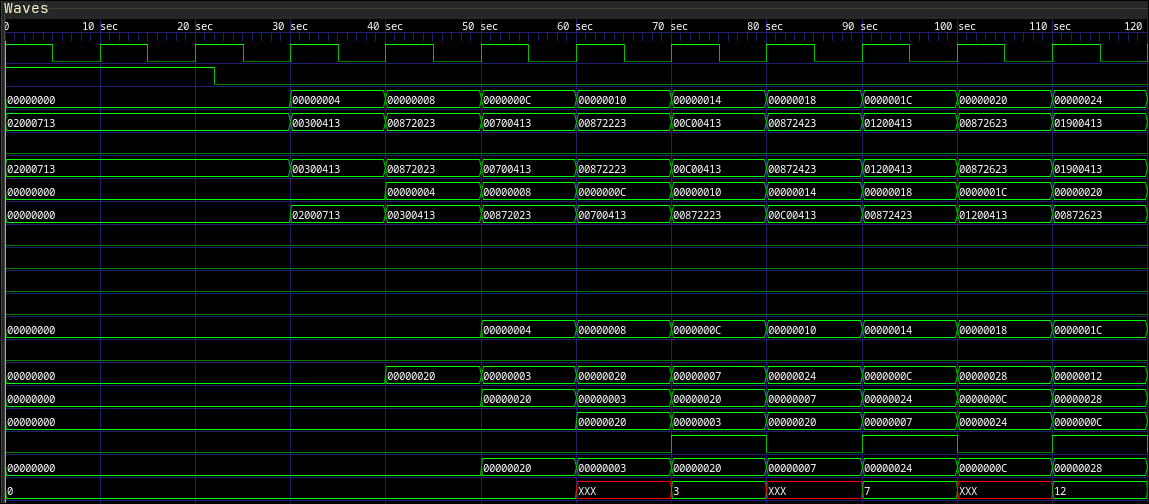
\includegraphics[width=\textwidth,height=0.72\textheight,keepaspectratio]{../../waves/bsearch/capturas_gtkwave/1_setup.png}
  {\scriptsize El arreglo \texttt{[3,7,12,18,25]} se escribe en memoria:
  \texttt{sw} consecutivos hacia \texttt{Mem[32..48]}.}
\end{frame}

\begin{frame}{Explicación de resultados (2/5): fin de setup, inicio del loop}
  \centering
  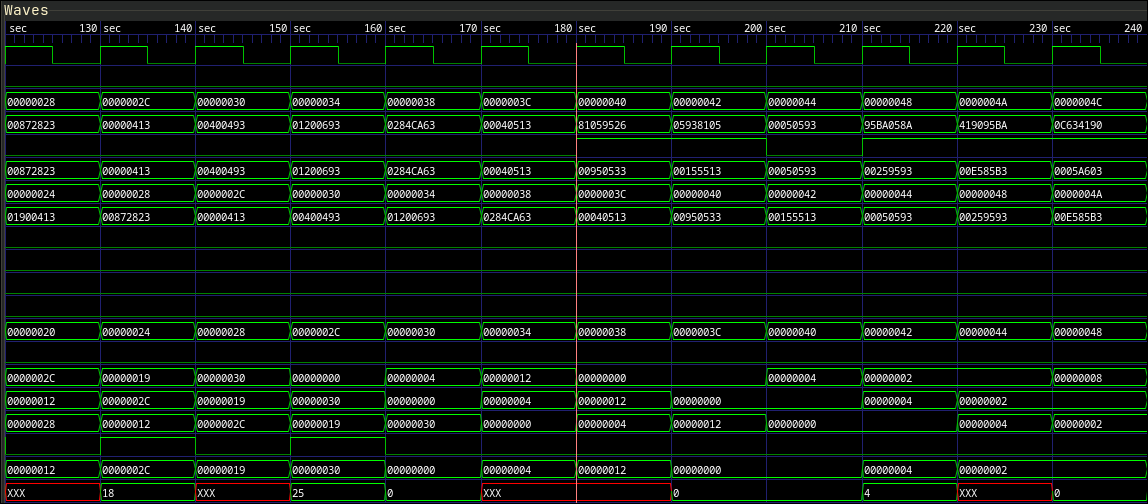
\includegraphics[width=\textwidth,height=0.72\textheight,keepaspectratio]{../../waves/bsearch/capturas_gtkwave/2_fin_setup_inicio_loop.png}
  {\scriptsize Últimos elementos del arreglo escritos; se inicializan
  \texttt{lo}, \texttt{hi}, \texttt{target} y el puntero de log --- entra al
  \texttt{LOOP}.}
\end{frame}

\begin{frame}{Explicación de resultados (3/5): iteración 1}
  \centering
  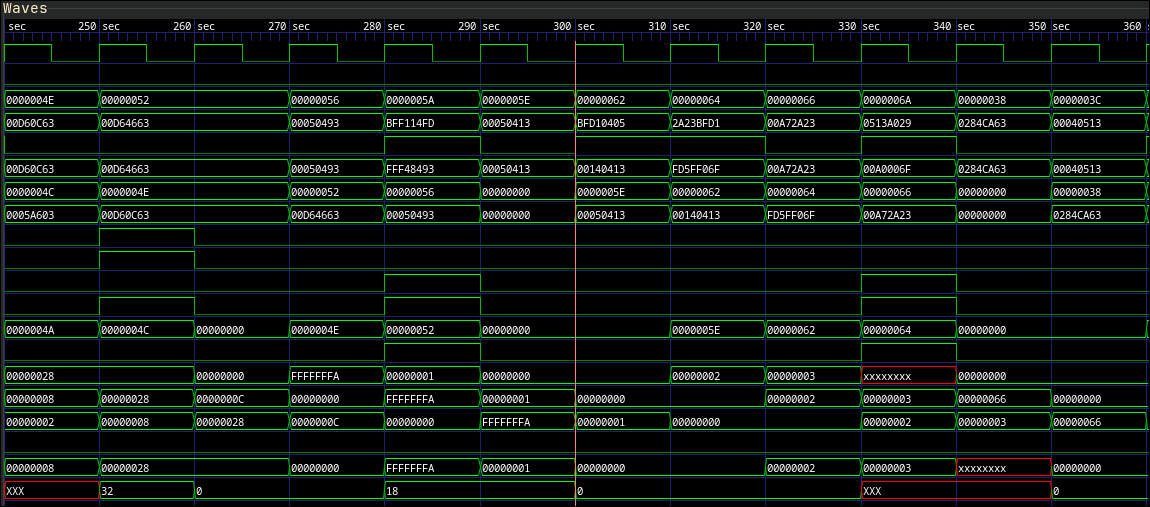
\includegraphics[width=\textwidth,height=0.72\textheight,keepaspectratio]{../../waves/bsearch/capturas_gtkwave/3_iteracion1_stall.png}
  {\scriptsize Cálculo de \texttt{mid}, lectura de \texttt{arr[mid]} con
  \texttt{c.lw} y comparación inmediata en \texttt{beq} --- el load-use
  hazard real, resuelto por la misma Hazard Unit del Capítulo 2.}
\end{frame}

\begin{frame}{Explicación de resultados (4/5): iteración 2}
  \centering
  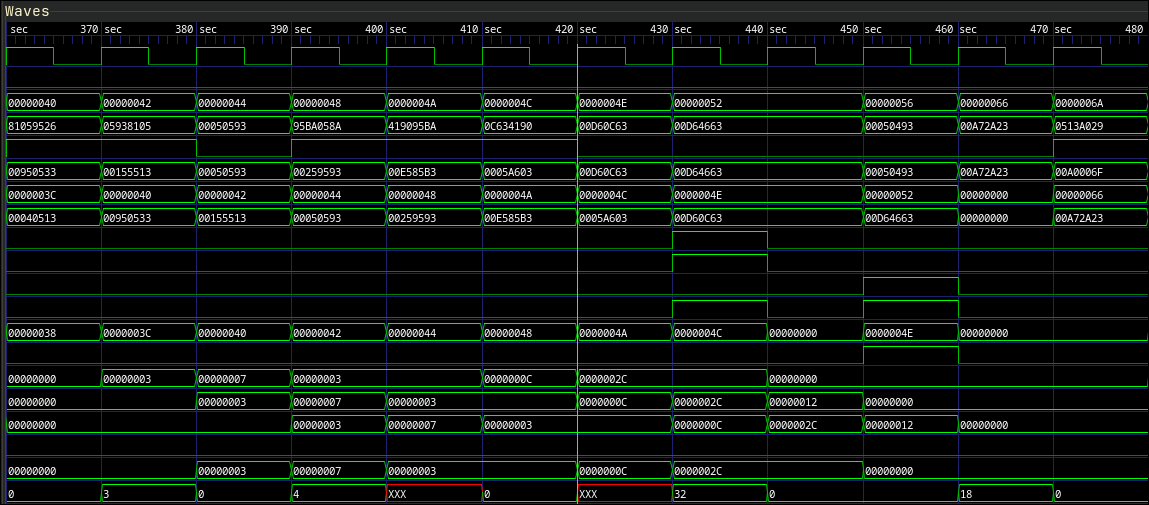
\includegraphics[width=\textwidth,height=0.72\textheight,keepaspectratio]{../../waves/bsearch/capturas_gtkwave/4_iteracion2.png}
  {\scriptsize Segunda vuelta del loop: nuevo \texttt{mid}, nueva lectura de
  memoria, nueva comparación --- el mismo patrón de la iteración 1, ahora
  con \texttt{lo}/\texttt{hi} actualizados.}
\end{frame}

\begin{frame}{Explicación de resultados (5/5): encontrado}
  \centering
  \noindent\makebox[\linewidth][c]{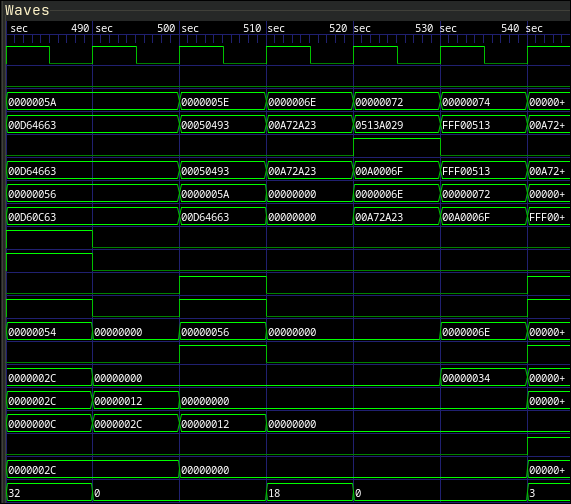
\includegraphics[width=\textwidth,height=0.72\textheight,keepaspectratio]{../../waves/bsearch/capturas_gtkwave/5_resultado.png}}
  {\scriptsize \texttt{arr[mid]==target} $\to$ encontrado. \texttt{Mem[52]=3}:
  el índice correcto de \texttt{18} en \texttt{[3,7,12,18,25]}.}
\end{frame}

\begin{frame}{Comparativa: \textit{performance}}
  \begin{block}{Hecho medido}
    RV32I puro y RVC: \textbf{545 ciclos en ambas} versiones (mismo
    algoritmo, mismo resultado).
  \end{block}
  \begin{exampleblock}{Razón}
    El descompresor es combinacional y vive \textbf{antes} del registro
    IF/ID --- no agrega etapas ni ciclos. Ninguna instrucción cuesta más por
    estar comprimida.
  \end{exampleblock}
  \begin{alertblock}{Execution Time}
    \centering \texttt{Execution Time = \#instrucciones × CPI × Tc} \\
    \small Los tres términos son iguales en ambas versiones: mismo
    \#instrucciones, mismo CPI, mismo Tc.
  \end{alertblock}
\end{frame}

\begin{frame}{Comparativa: tamaño}
  De 37 instrucciones totales (mismo algoritmo en ambas versiones):
  \begin{table}
    \centering
    \small
    \begin{tabular}{@{}lccc@{}}
      \toprule
      \textbf{Versión} & \textbf{Instr. 32b} & \textbf{Instr. 16b} & \textbf{Bytes} \\
      \midrule
      RV32I puro & 37 & 0 & $37\times4=148$ \\
      Con RVC & 25 & 12 & $25\times4+12\times2=124$ \\
      \bottomrule
    \end{tabular}
  \end{table}
  \begin{center}
    \textbf{12 de 37 instrucciones comprimidas (32\,\%) $\to$ 24 bytes
    ahorrados (16\,\% menos código)}, con cero costo en ciclos.
  \end{center}
\end{frame}

% ============================================================
\section{Conclusiones}
% ============================================================

\begin{frame}{Conclusiones}
  \begin{itemize}
    \item<1-> Pipeline de 5 etapas completo (RV32I, 24 instrucciones) +
      Hazard Unit funcional, validada con y sin ella (falla sin, funciona
      con).
    \item<2-> Extensión RVC (21 instrucciones, E2+E3) integrada
      \textbf{sin modificar} pipeline/control/hazard unit --- todo resuelto
      en un descompresor combinacional antes de IF/ID.
    \item<3-> Validación incremental por fases, regresión completa en verde
      (26/26 tests).
    \item<4-> \texttt{bsearch} demuestra todo integrado a la vez: pipeline +
      hazard unit + RVC funcionando juntos, con 16\,\% menos código y cero
      costo en ciclos.
  \end{itemize}
\end{frame}

\begin{frame}{Desafíos reales}
  \begin{itemize}
    \item<1-> \textbf{Timing del regfile (E1)}: con dependencia a distancia
      3 (WB y Decode en el mismo ciclo), el regfile genérico
      (\texttt{posedge}) no hacía visible el dato a tiempo. Corregido con
      \textbf{write-first en \texttt{negedge}} (Harris \& Harris, Sec.
      7.5.1) --- puente hacia el forwarding.
    \item<2-> \textbf{Bug real en \texttt{c.lw} (E3)}: el destino vive en
      \texttt{c[4:2]}, no en \texttt{c[9:7]} como sugería la analogía con
      CB. Depurado aislando el \texttt{decompressor.v} del resto del
      pipeline.
    \item<3-> \textbf{Volumen de archivos}: más de 25 pares
      \texttt{.mem}/testbench --- mantenerlos sincronizados fue un desafío
      de organización tanto como de diseño.
  \end{itemize}
\end{frame}

\begin{frame}{Mejoras futuras}
  \begin{itemize}
    \item<1-> Ampliar el subset de RVC (\texttt{c.li}, \texttt{c.addi16sp},
      \texttt{c.addi4spn}) y agregar detección de encoding ilegal (trap),
      hoy ausente.
    \item<2-> \textbf{Predicción de branches}: cada salto tomado paga el
      costo de \textit{flush} (visible en el waveform de \texttt{bsearch});
      una predicción estática simple (\textit{backward=taken}) acercaría el
      CPI real al ideal de 1.
  \end{itemize}
\end{frame}

\begin{frame}
  \centering
  \Huge Gracias
  \vspace{0.5cm}

  
\includegraphics[height=0.55\textheight]{../fgsfds-osaka.png}
\end{frame}

\end{document}
